% Options for packages loaded elsewhere
\PassOptionsToPackage{unicode}{hyperref}
\PassOptionsToPackage{hyphens}{url}
%
\documentclass[
]{article}
\usepackage{amsmath,amssymb}
\usepackage{iftex}
\ifPDFTeX
  \usepackage[T1]{fontenc}
  \usepackage[utf8]{inputenc}
  \usepackage{textcomp} % provide euro and other symbols
\else % if luatex or xetex
  \usepackage{unicode-math} % this also loads fontspec
  \defaultfontfeatures{Scale=MatchLowercase}
  \defaultfontfeatures[\rmfamily]{Ligatures=TeX,Scale=1}
\fi
\usepackage{lmodern}
\ifPDFTeX\else
  % xetex/luatex font selection
\fi
% Use upquote if available, for straight quotes in verbatim environments
\IfFileExists{upquote.sty}{\usepackage{upquote}}{}
\IfFileExists{microtype.sty}{% use microtype if available
  \usepackage[]{microtype}
  \UseMicrotypeSet[protrusion]{basicmath} % disable protrusion for tt fonts
}{}
\makeatletter
\@ifundefined{KOMAClassName}{% if non-KOMA class
  \IfFileExists{parskip.sty}{%
    \usepackage{parskip}
  }{% else
    \setlength{\parindent}{0pt}
    \setlength{\parskip}{6pt plus 2pt minus 1pt}}
}{% if KOMA class
  \KOMAoptions{parskip=half}}
\makeatother
\usepackage{xcolor}
\usepackage{graphicx}
\makeatletter
\def\maxwidth{\ifdim\Gin@nat@width>\linewidth\linewidth\else\Gin@nat@width\fi}
\def\maxheight{\ifdim\Gin@nat@height>\textheight\textheight\else\Gin@nat@height\fi}
\makeatother
% Scale images if necessary, so that they will not overflow the page
% margins by default, and it is still possible to overwrite the defaults
% using explicit options in \includegraphics[width, height, ...]{}
\setkeys{Gin}{width=\maxwidth,height=\maxheight,keepaspectratio}
% Set default figure placement to htbp
\makeatletter
\def\fps@figure{htbp}
\makeatother
\setlength{\emergencystretch}{3em} % prevent overfull lines
\providecommand{\tightlist}{%
  \setlength{\itemsep}{0pt}\setlength{\parskip}{0pt}}
\setcounter{secnumdepth}{-\maxdimen} % remove section numbering
\ifLuaTeX
  \usepackage{selnolig}  % disable illegal ligatures
\fi
\IfFileExists{bookmark.sty}{\usepackage{bookmark}}{\usepackage{hyperref}}
\IfFileExists{xurl.sty}{\usepackage{xurl}}{} % add URL line breaks if available
\urlstyle{same}
\hypersetup{
  hidelinks,
  pdfcreator={LaTeX via pandoc}}

\author{}
\date{}

\begin{document}

\tableofcontents

\subsubsection{Task 4 : Introduce the SA, the standard BGA and the
improved
BGA.}\label{task-4---introduce-the-sa-the-standard-bga-and-the-improved-bga}

\paragraph{Simulated Annealing}\label{simulated-annealing}

\subparagraph{\texorpdfstring{Pseudocode
}{Pseudocode }}\label{pseudocode}

\subparagraph{Flowchart}\label{flowchart}

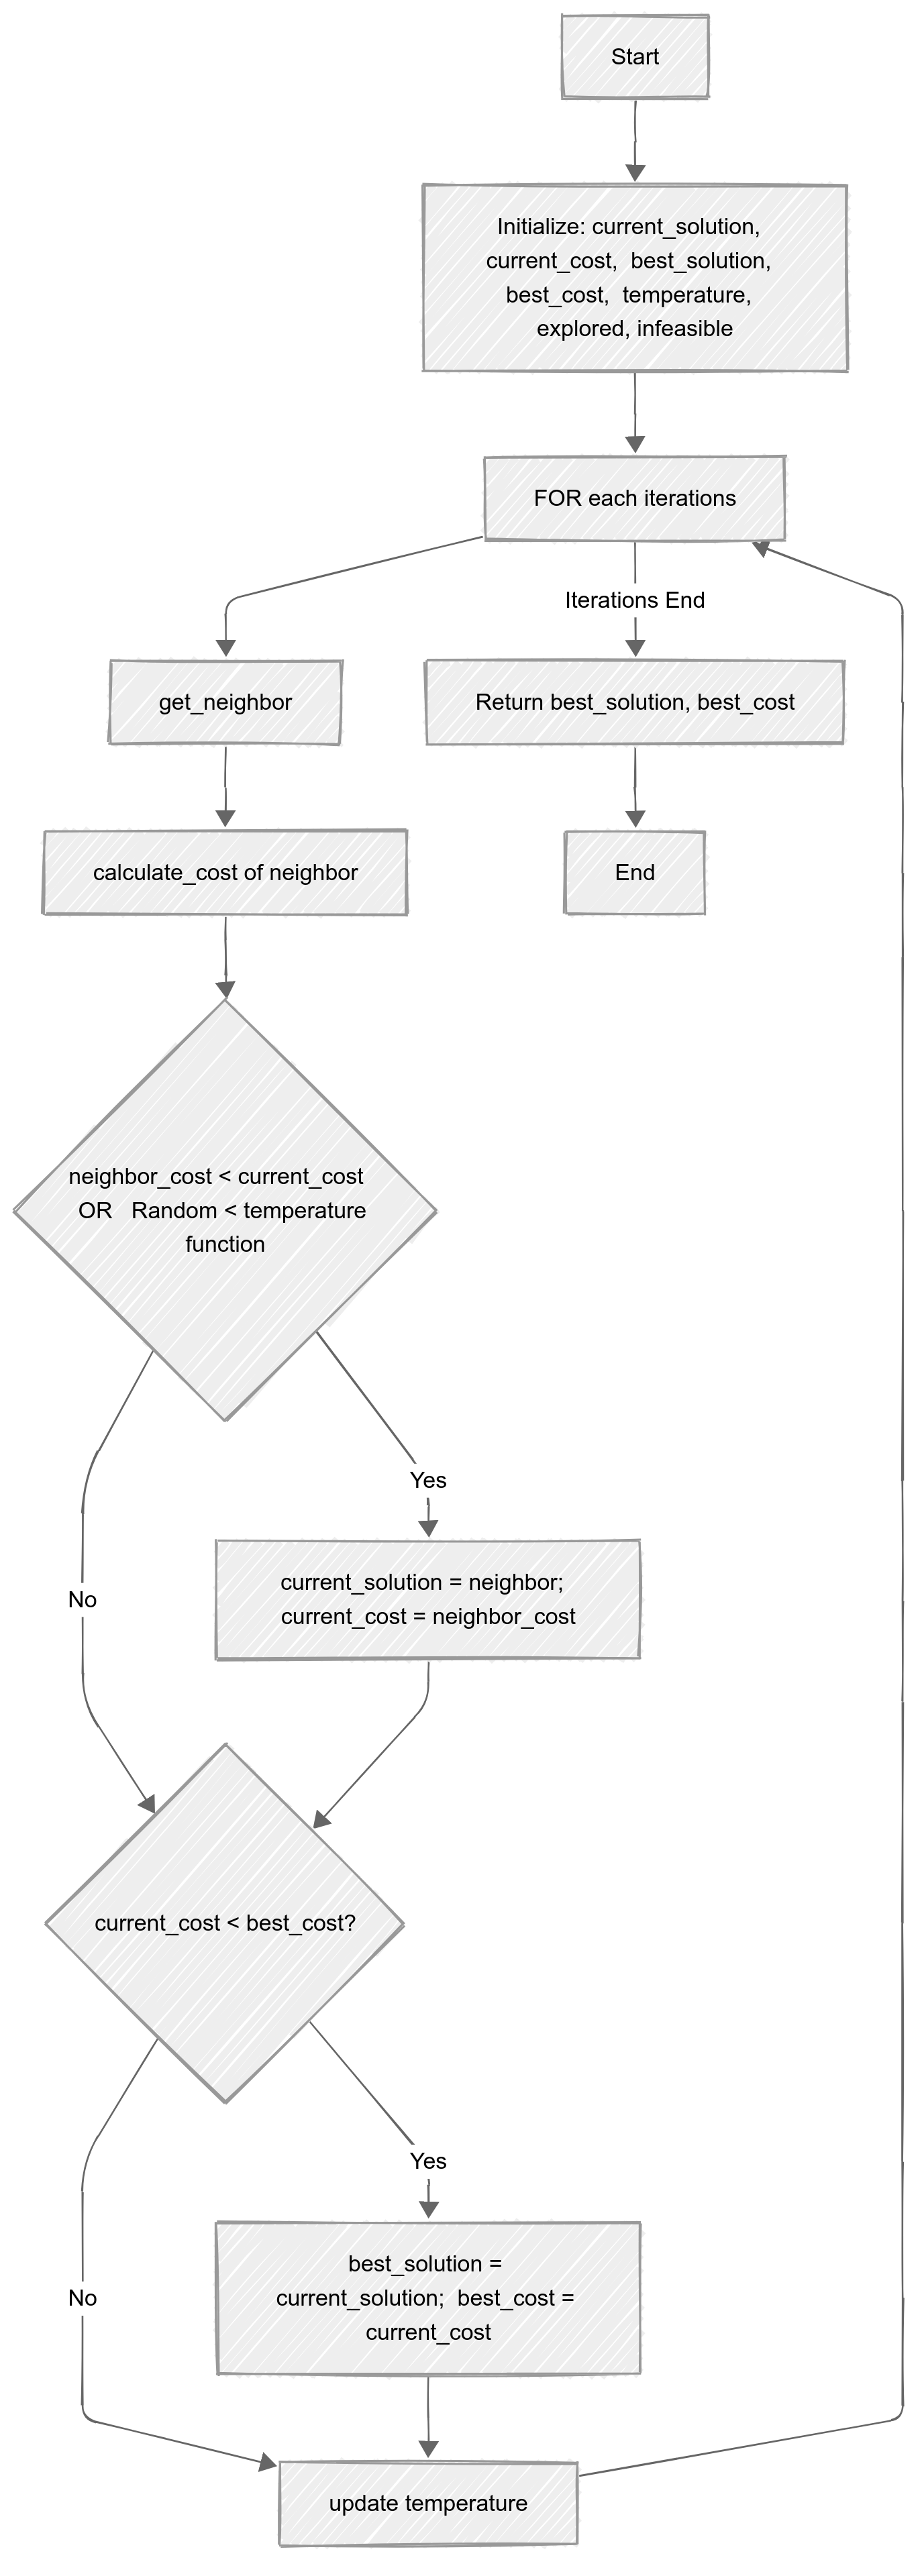
\includegraphics{/home/violetboy/media/partition2/sync/iit-codiing/UoB-EC/simulated_annealing2.png}

\paragraph{Standard - BGA}\label{standard---bga}

\subparagraph{Pseudo code}\label{pseudo-code}

\subparagraph{Flowchart}\label{flowchart-2}

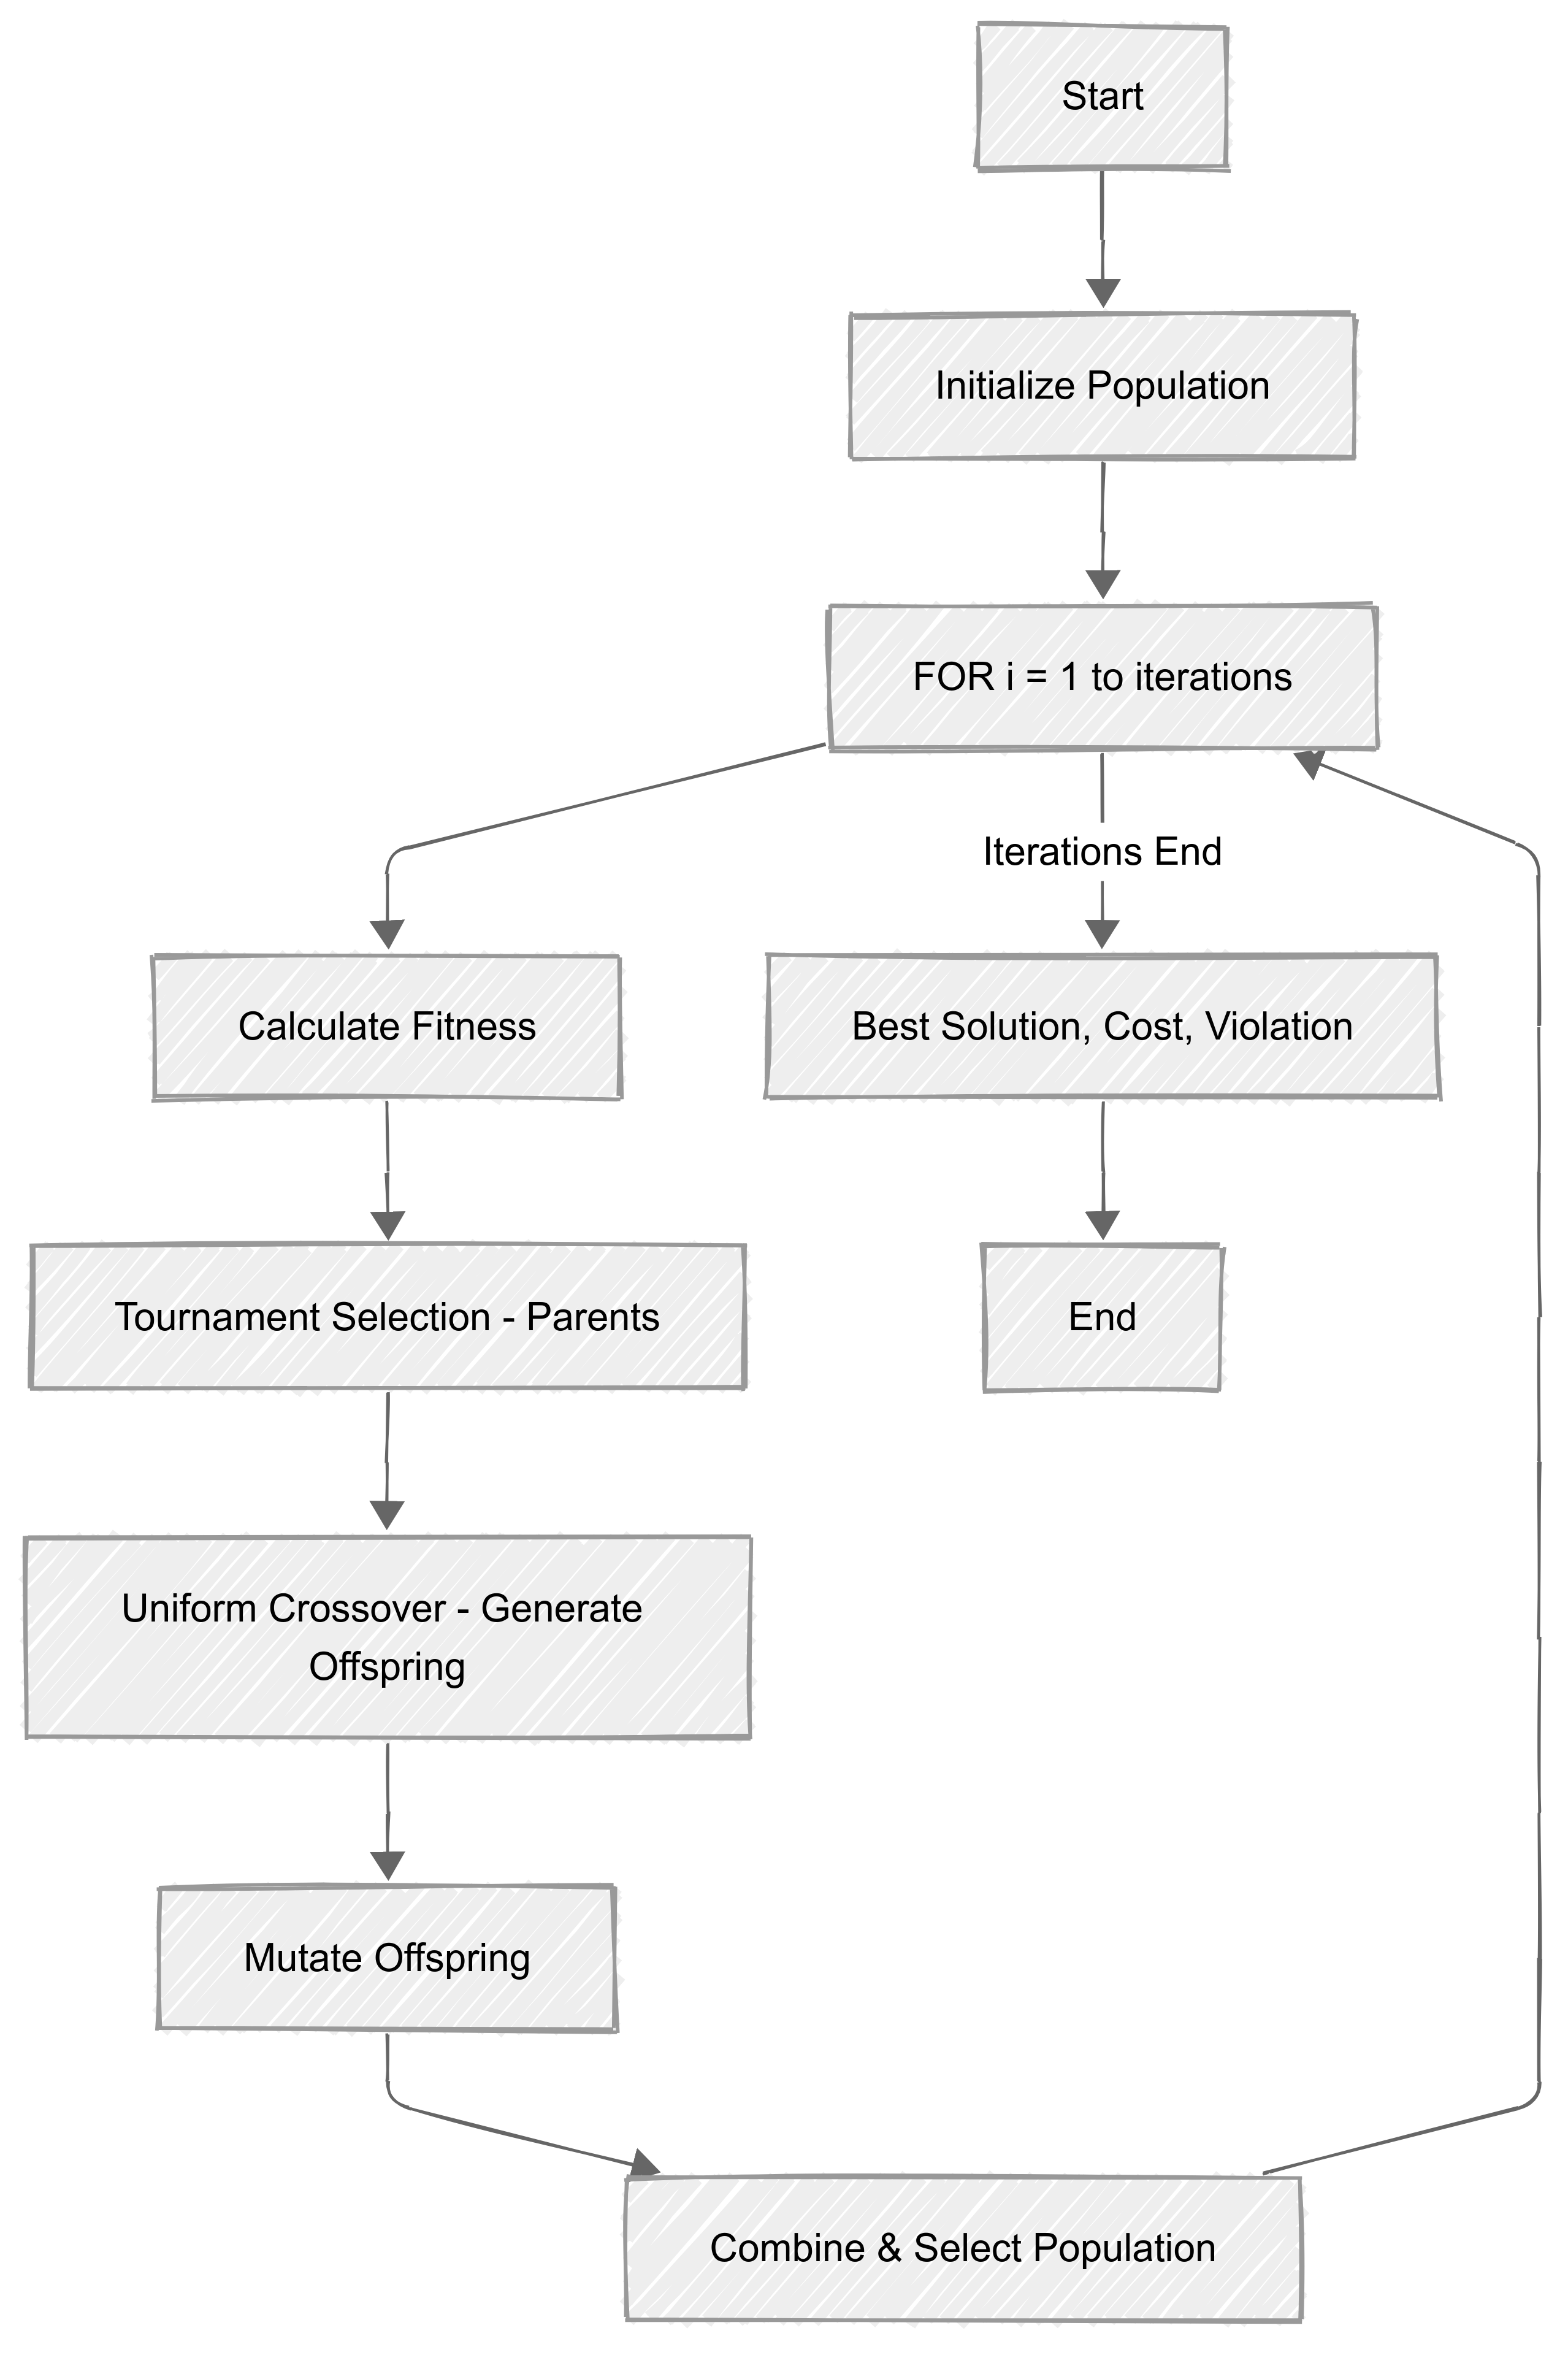
\includegraphics{/home/violetboy/media/partition2/sync/iit-codiing/UoB-EC/standard_bga.png}

\paragraph{Improved - BGA}\label{improved---bga}

\subparagraph{Pseudo code}\label{pseudo-code-2}

\subparagraph{Flowchart}\label{flowchart-3}

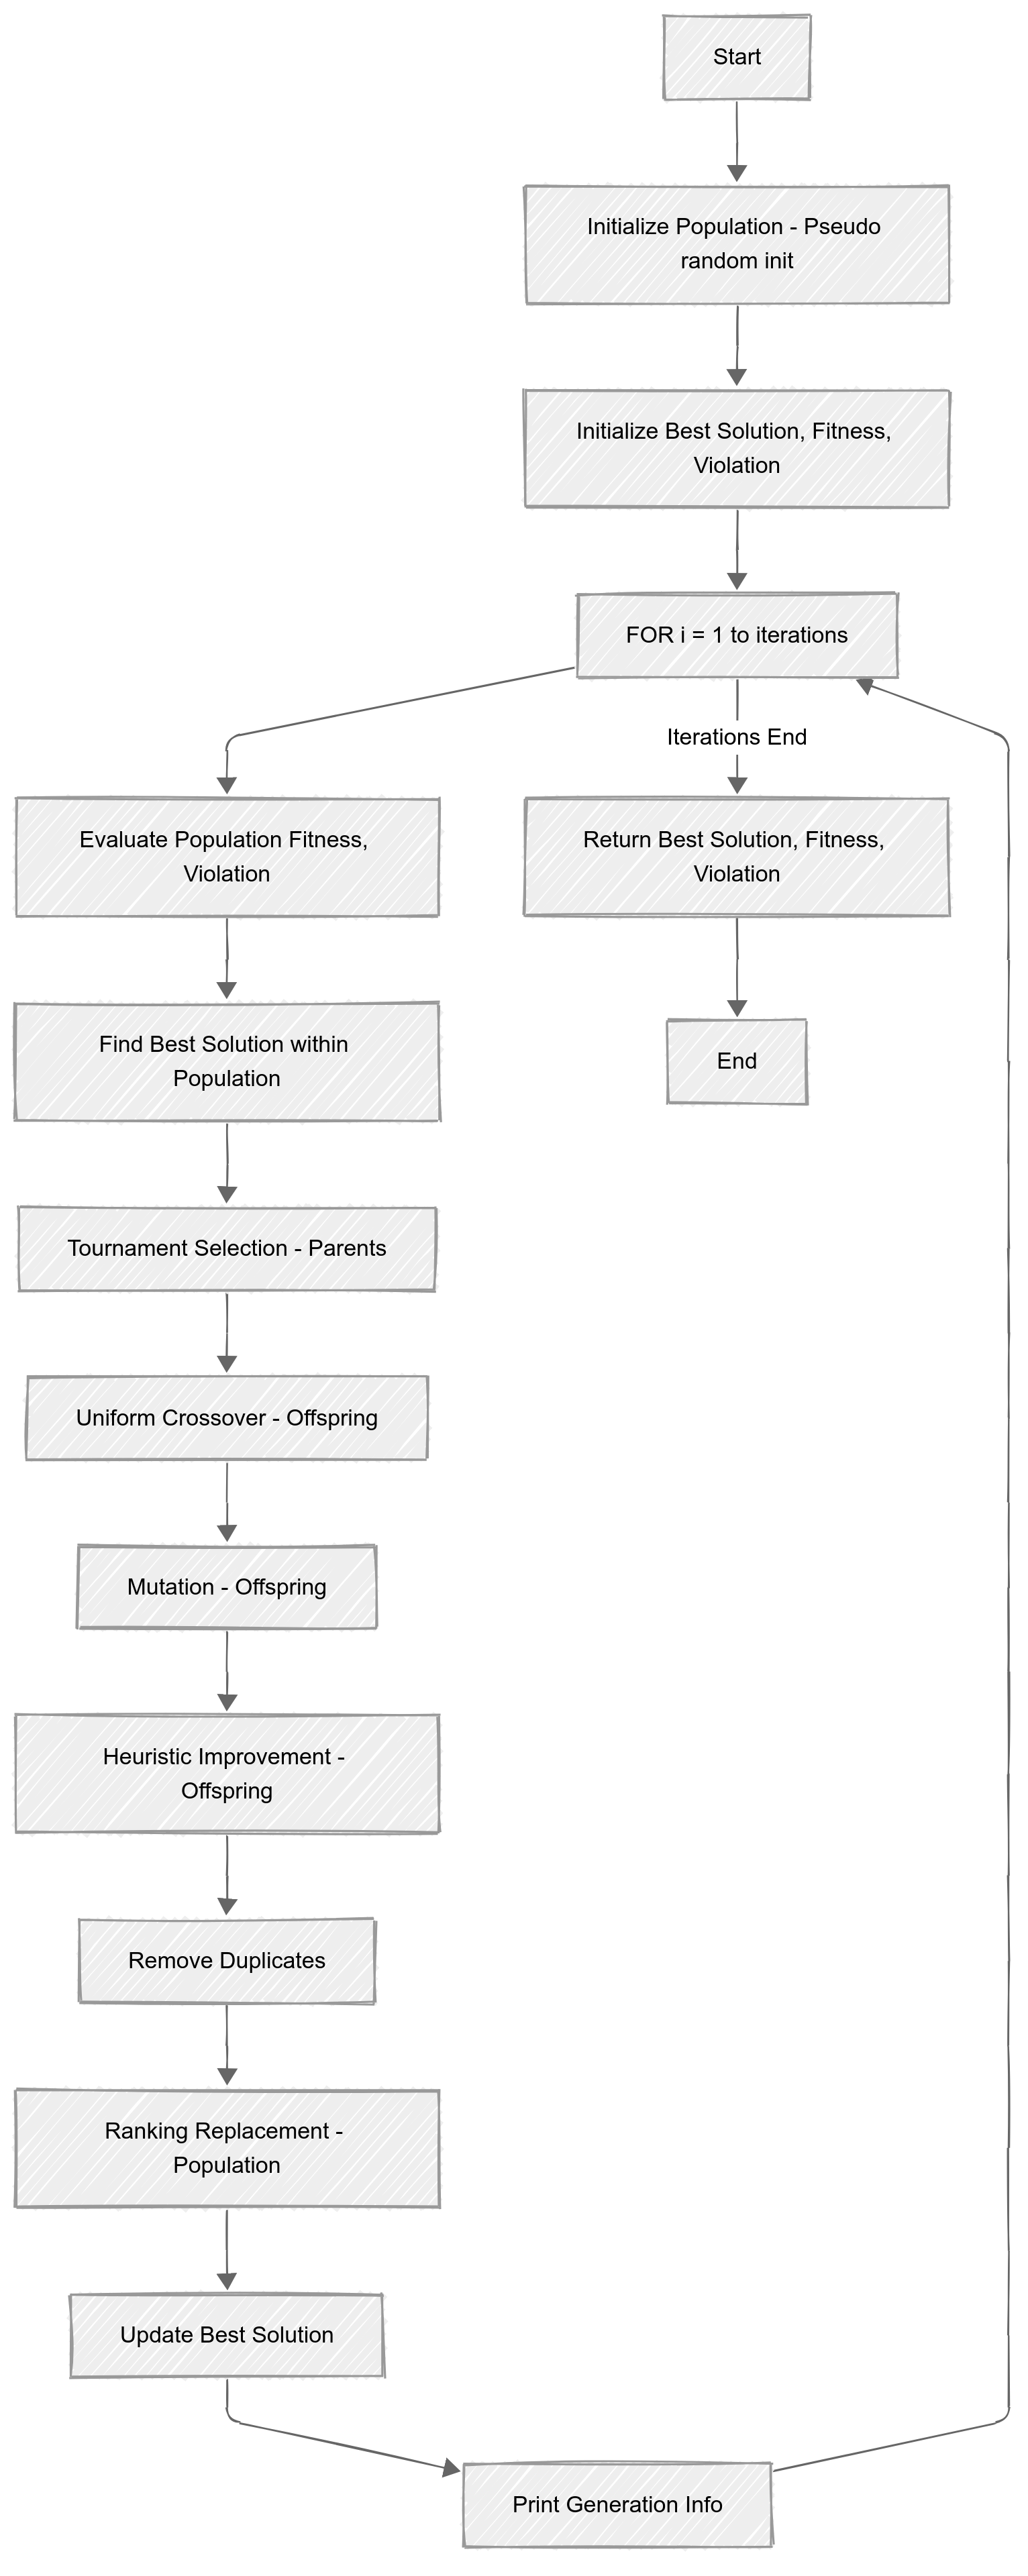
\includegraphics{/home/violetboy/media/partition2/sync/iit-codiing/UoB-EC/improved_bga.png}

\subsubsection{Task 5 : For each benchmark problem, list the average
result and standard deviations obtained over 30 independent runs of each
algorithm.}\label{task-5--for-each-benchmark-problem-list-the-average-result-and-standard-deviations-obtained-over-30-independent-runs-of-each-algorithm}

\subparagraph{Result Table}\label{result-table}

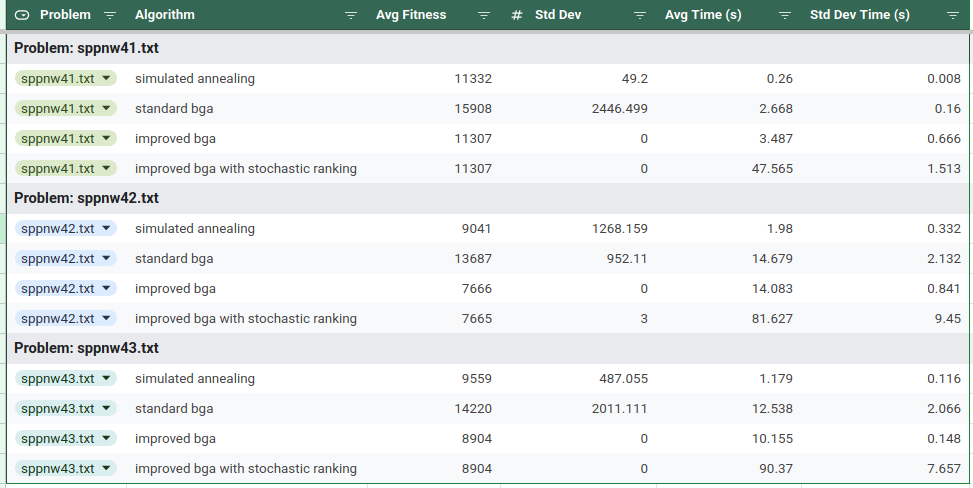
\includegraphics{/home/violetboy/media/partition2/sync/iit-codiing/UoB-EC/image-20250307211416070.png}

\subsubsection{\texorpdfstring{Task 6 : Similarity and difference
between the ranking replacement method and the stochastic ranking method
}{Task 6 : Similarity and difference between the ranking replacement method and the stochastic ranking method }}\label{task-6--similarity-and-difference-between-the-ranking-replacement-method-and-the-stochastic-ranking-method}

\begin{itemize}
\item ~
  \subparagraph{Difference}\label{difference}

  \begin{itemize}
  \item
    Ranking Replacement focuses on the \textbf{selection} of individuals
    for deletion after offspring are produced, acts like a replacement
    algorithm.
  \item
    Stochastic Ranking focuses on the \textbf{ordering} ranking/sorting
    of the population, acts like a sorting algorithm. Other than
    unfitness and fitness value, Stochastic Ranking has \(p_f\)
    probabilistic value , through which (\(p_f<0.5\)) we can prioritise
    feasible solutions (zero constraint violation) while allowing
    exploration of infeasible regions.
  \end{itemize}
\item ~
  \subparagraph{Similarity}\label{similarity}

  \begin{itemize}
  \item
    Both handles constraint violation.
  \item
    Both considers unfitness(constraint violation) and fitness
    value(objective function).
  \end{itemize}
\end{itemize}

\subsubsection{Task 7 : Compare the results from SA, the standard BGA
and the improved BGA with an in-depth
discussion.}\label{task-7---compare-the-results-from-sa-the-standard-bga-and-the-improved-bga-with-an-in-depth-discussion}

\subparagraph{Experiment details :}\label{experiment-details-}

\begin{itemize}
\item
  trials : 30 (independent)
\item
  Standard BGA

  \begin{itemize}
  \item
    initial population size :1000
  \item
    Iteration : 100
  \end{itemize}
\item
  Improved BGA and Imporved BGA with Stochastic ranking

  \begin{itemize}
  \item
    initial population size :100
  \item
    Iteration : 100
  \end{itemize}
\end{itemize}

\paragraph{Overall Observations:}\label{overall-observations}

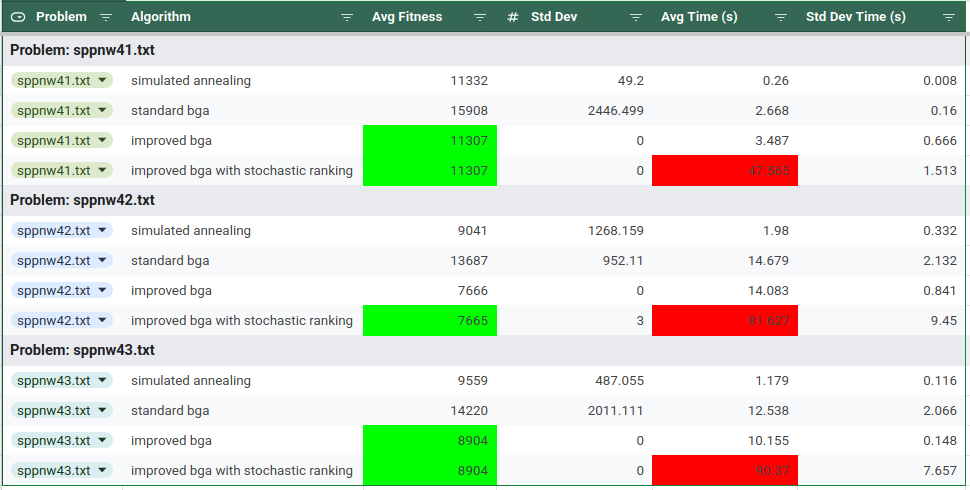
\includegraphics{/home/violetboy/media/partition2/sync/iit-codiing/UoB-EC/image-20250307214405822.png}

\subparagraph{Fitness score analysis}\label{fitness-score-analysis}

\textbf{Improved Genetic Algorithms (ibga and ibgasr)}: Across all three
benchmark problems (sppnw41.txt, sppnw42.txt, sppnw43.txt), the improved
basic genetic algorithm (ibga) and the improved basic genetic algorithm
with stochastic ranking (ibgasr) consistently \textbf{achieve the lowest
average fitness values}. This indicates that the enhancements made to
the basic genetic algorithm are highly effective in finding better
solutions.

\textbf{Stochastic Annealing (sa) is Competitive:} Simulated annealing
(sa) demonstrates competitive performance, particularly on sppnw41.txt,
where it achieves results comparable to the improved genetic algorithms.
However, its performance is less consistent across other problems.

\textbf{Basic Genetic Algorithm (bga) is Outperformed:} The standard
basic genetic algorithm (bga) is consistently outperformed by all other
algorithms in terms of solution quality (average fitness). This
highlights the importance of incorporating improvements or alternative
search strategies.

\textbf{Impact of Stochastic Ranking (ibgasr):} In terms of average
fitness, the addition of stochastic ranking (ibgasr) to the improved
genetic algorithm does not significantly affect the solution quality.
However, it does have a noticeable impact on the execution time ie
higher execution time.

\subparagraph{Execution Time Variation}\label{execution-time-variation}

There are substantial differences in execution time between the
algorithms. The improved genetic algorithms (ibgasr) generally take
longer than than other algorithm considered, likely due to the
additional computational overhead of the stochastic ranking process.

\subparagraph{Standard Deviation
Analysis}\label{standard-deviation-analysis}

The improved genetic algorithms (ibga and ibgasr) show very low or zero
standard deviations in fitness, indicating \textbf{high consistency in
solution quality} across multiple runs. Simulated annealing (sa) and the
basic genetic algorithm (bga) exhibit higher standard deviations,
suggesting greater variability in solution quality across runs.

\subparagraph{Initial population size}\label{initial-population-size}

For Standard BGA initial population size of 1000 is kept for faster
convergence with 100 iterations. Where improved BGA required only
initial population of 100 is required and converged in less than 30
iterations

\paragraph{Summary}\label{summary}

\begin{itemize}
\item
  The improved genetic algorithms demonstrate superior performance in
  terms of solution quality and consistency.
\item
  Stochastic annealing offers a viable alternative, especially when
  execution time is a concern.
\item
  Adding stochastic ranking increases runtime.
\end{itemize}

\end{document}
